\documentclass{classrep}
\usepackage[utf8]{inputenc}
\frenchspacing

\usepackage{graphicx}
\usepackage[usenames,dvipsnames]{color}
\usepackage[hidelinks]{hyperref}
\usepackage{lmodern}
\usepackage{graphicx}
\usepackage{placeins}
\usepackage{url}
\usepackage{amsmath, amssymb, mathtools}
\usepackage{listings}
\usepackage{fancyhdr, lastpage}

\pagestyle{fancyplain}
\fancyhf{}
\renewcommand{\headrulewidth}{0pt}
\cfoot{\thepage\ / \pageref*{LastPage}}

\studycycle{Informatyka Stosowana, studia dzienne, inż I st.}
\coursesemester{IV}

\coursename{Sztuczna inteligencja i systemy ekspertowe}
\courseyear{2022/2023}

\courseteacher{dr inż. Krzysztof Lichy}
\coursegroup{poniedziałek, 15:45}

\author{
  \studentinfo{Marcin Giska}{242390} \and
  \studentinfo{Przemysław Musiał}{242473}
}

\title{Zadanie 1: Piętnastka}

\begin{document}
    \maketitle
    \thispagestyle{fancyplain}

    \section{Cel} {
    Celem części programistycznej jest napisanie programu, który będzie rozwiązywał "Piętnastkę". Cel części badawczej stanowi przebadanie, jak metody przeszukiwania przestrzeni stanów zachowują się w przypadku tego problemu.
    }

    \section{Wprowadzenie} {
    Łamigłówka „Piętnastka” jest układanką składającą się z ramki i osadzonych w niej 15 elementów, kwadratowej planszy o wymiarach 4x4. Na każdym elemencie znajduje się numer od 1 do 15. Jedno miejsce jest puste, umożliwia ono przesuwanie elementów. Za stan rozwiązany przyjmuje się taki układ elementów, w którym są one ułożone rosnąco od lewej do prawej oraz od góry do dołu. Ułożenie układanki można potraktować jak przeszukiwanie drzewa składającego się z węzłów o wartościach „R”, „D”, „U” oraz „L” odpowiadających „przesunięciem” pustego pola w prawo, dół, górę oraz lewo.
    }

    \section{Opis implementacji} {
    Stworzona aplikacja rozwiązująca "Piętnastkę" została napisana w języku Python. Kod składa się z następujących definicji:
        \begin{itemize}
            \item DFS (maksymalna dozwolona głębokość rekursji przyjmuje wartość 20. W sytuacji, gdy program osiągnie taką głębokość i nie znajdzie rozwiązania, powinien wykonać nawrót)
            \item BFS
            \item ASTR
        \end{itemize}
    }

    \section{Materiały i metody} {
        Do wykonania zadania zostaly wykorzystane skrypty, które są dostępne na stronie przedmiotu. Dzięki tym skryptom zostało storzonych 413 układów. W przypadku strategii "wszerz" i strategii "w głąb" użyliśmy 8 następujących porządków przeszukiwania sąsiedztwa:
        \begin{itemize}
            \item prawo-dół-góra-lewo
            \item prawo-dół-lewo-góra
            \item dół-prawo-góra-lewo
            \item dół-prawo-lewo-góra
            \item lewo-góra-dół-prawo
            \item lewo-góra-prawo-dół
            \item góra-lewo-dół-prawo
            \item góra-lewo-prawo-dół
        \end{itemize}
        \bigskip
    Odpowiednie wykresy zostały wygenerowane za pomocą oddzielnego programu napisanemu w pythonie.
    }

    \section{Wyniki} {
        Wykresy zostały podzielone ze względu na strategię przeszukiwania

        \begin{figure}[!htbp]
            \centering
            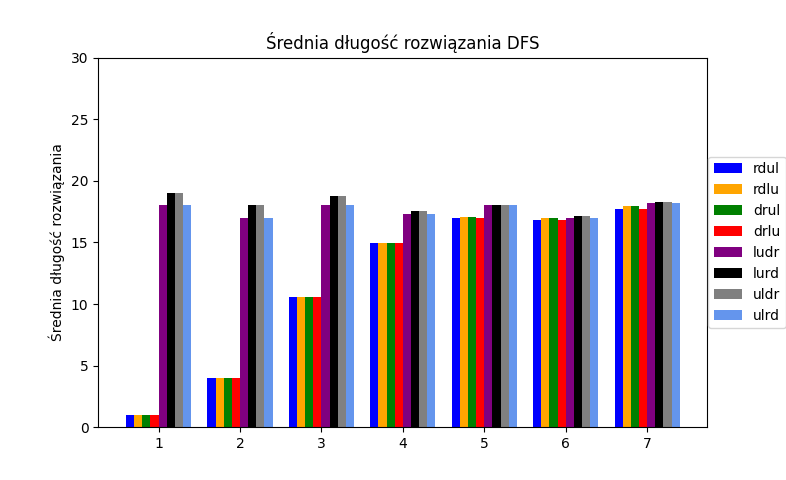
\includegraphics[width=\textwidth, height=70mm]{wykresy/dfs1.png}
            \caption{Średnia długość rozwiązania}
        \end{figure}

        \begin{figure}[!htbp]
            \centering
            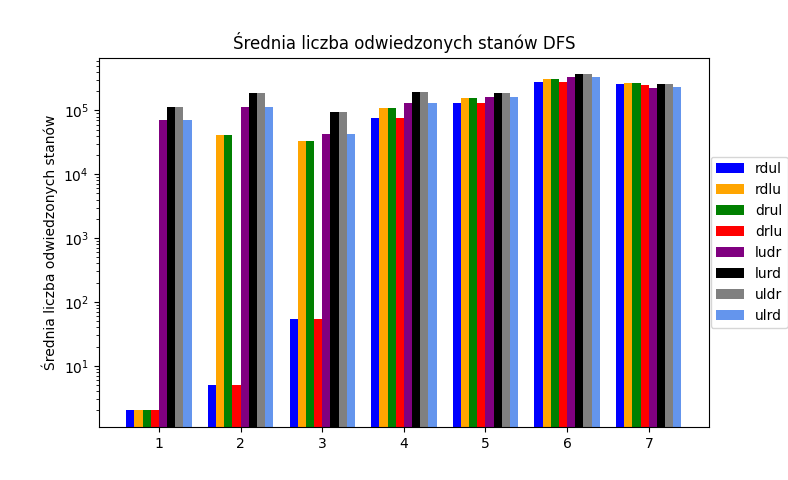
\includegraphics[width=\textwidth, height=55mm]{wykresy/dfs2.png}
            \caption{Średnia liczba odwiedzonych stanów}
        \end{figure}

         \begin{figure}[!htbp]
             \centering
            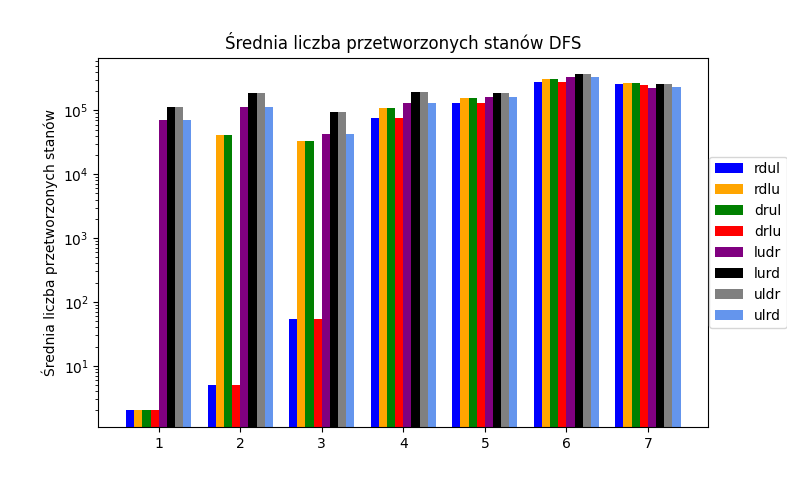
\includegraphics[width=\textwidth, height=55mm]{wykresy/dfs3.png}
            \caption{Średnia liczba przetworzonych stanów}
        \end{figure}

        \begin{figure}[!htbp]
             \centering
             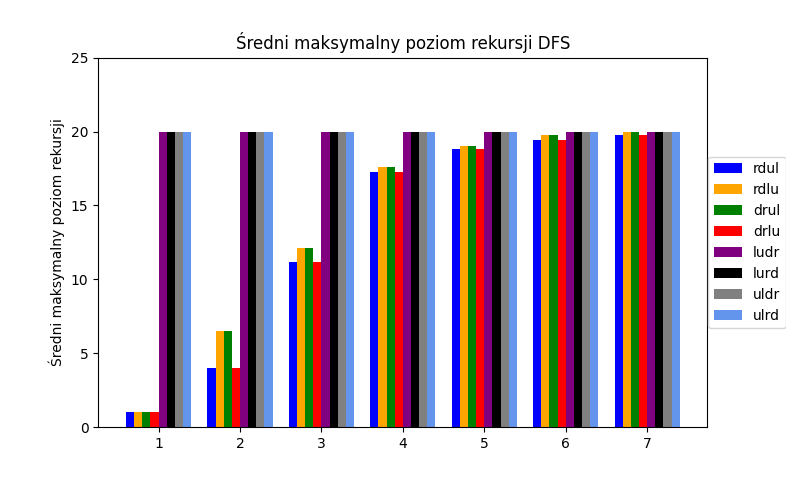
\includegraphics[width=\textwidth, height=55mm]{wykresy/dfs4.png}
             \caption{Średni maksymalny poziom rekursji}
        \end{figure}

        \begin{figure}[!htbp]
            \centering
            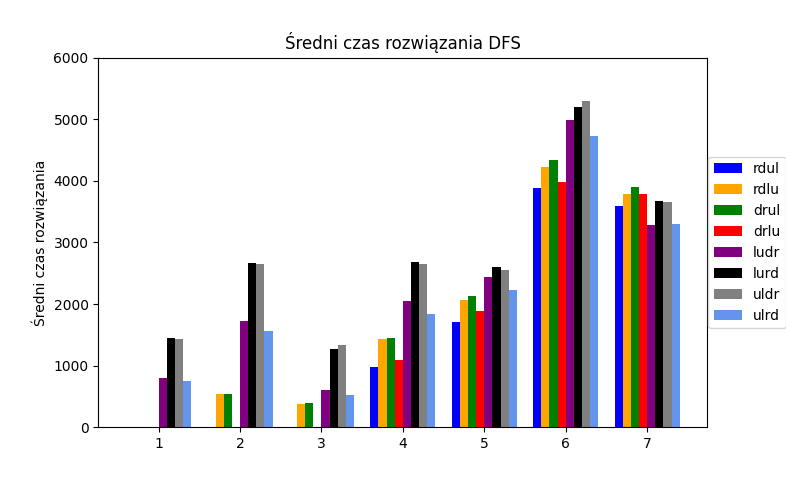
\includegraphics[width=\textwidth, height=55mm]{wykresy/dfs5.png}
            \caption{Średni czas rozwiązania}
        \end{figure}
        \FloatBarrier

        

        \begin{figure}[!htbp]
            \centering
            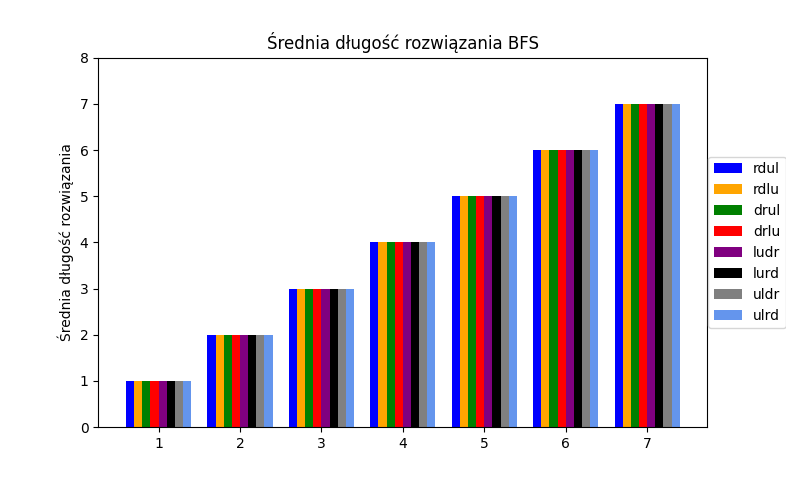
\includegraphics[width=\textwidth, height=55mm]{wykresy/bfs1.png}
            \caption{Średnia długość rozwiązania}
        \end{figure}

        \begin{figure}[!htbp]
            \centering
            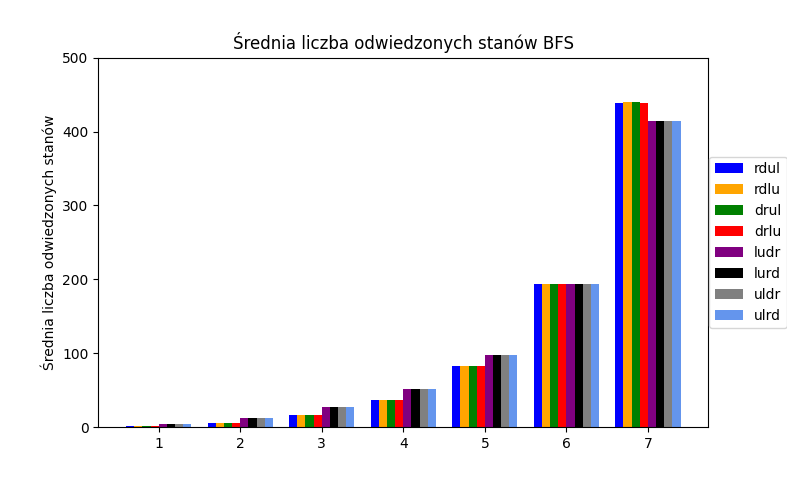
\includegraphics[width=\textwidth, height=55mm]{wykresy/bfs2.png}
            \caption{Średnia liczba odwiedzonych stanów}
        \end{figure}

        \begin{figure}[!htbp]
            \centering
            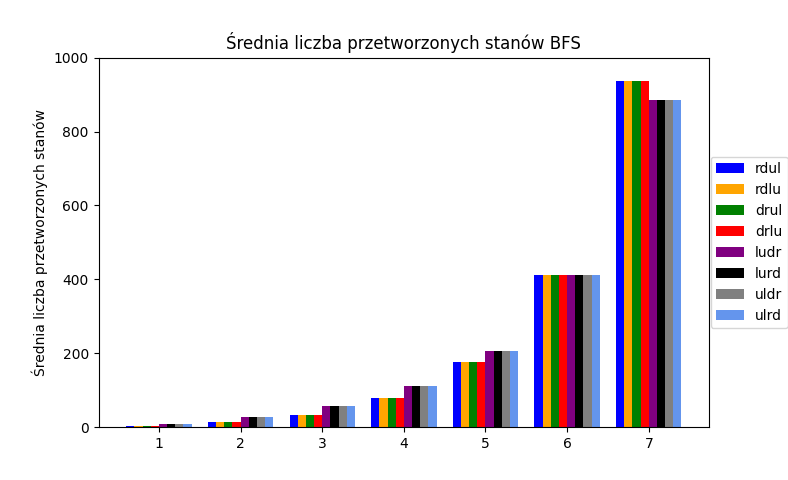
\includegraphics[width=\textwidth, height=55mm]{wykresy/bfs3.png}
            \caption{Średnia liczba przetworzonych stanów}
        \end{figure}

        \begin{figure}[!htbp]
            \centering
            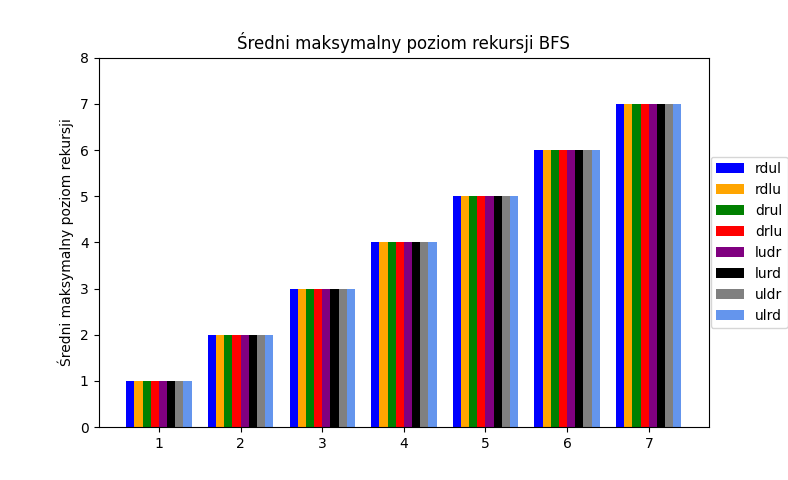
\includegraphics[width=\textwidth, height=55mm]{wykresy/bfs4.png}
            \caption{Średni maksymalny poziom rekursji}
        \end{figure}

        \begin{figure}[!htbp]
            \centering
            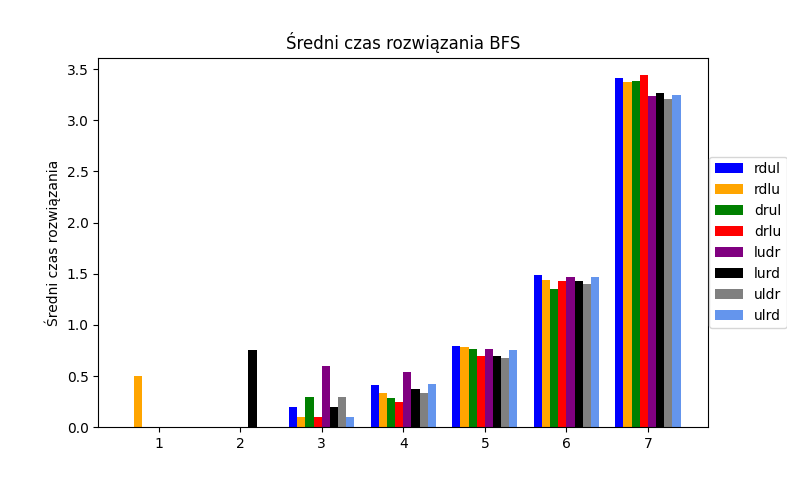
\includegraphics[width=\textwidth, height=55mm]{wykresy/bfs5.png}
            \caption{Średni czas rozwiązania}
        \end{figure}
        \FloatBarrier

        

        \begin{figure}[!htbp]
            \centering
            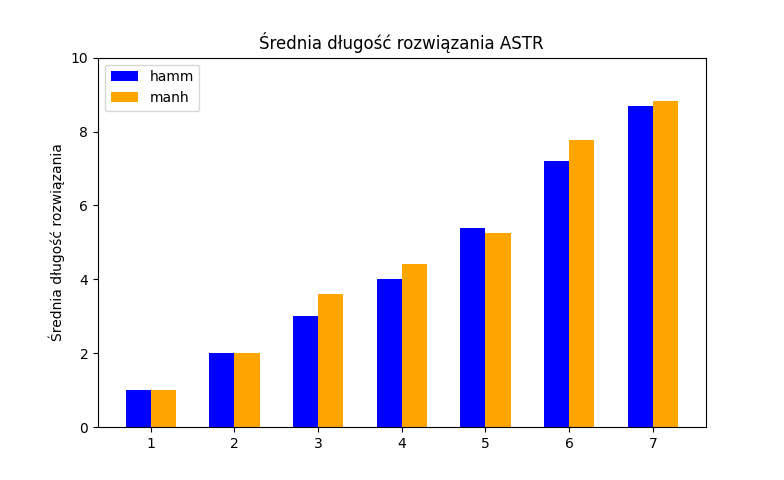
\includegraphics[width=\textwidth, height=55mm]{wykresy/astr1.png}
            \caption{Średnia długość rozwiązania}
        \end{figure}

        \begin{figure}[!htbp]
            \centering
            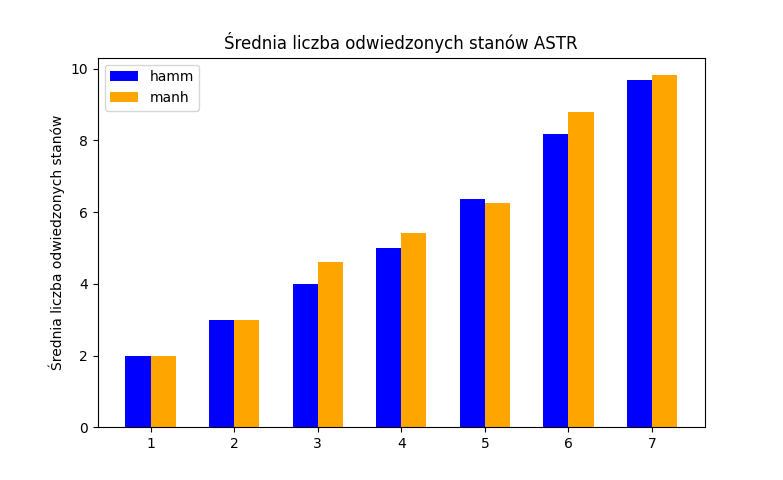
\includegraphics[width=\textwidth, height=55mm]{wykresy/astr2.png}
            \caption{Średnia liczba odwiedzonych stanów}
        \end{figure}

        \begin{figure}[!htbp]
            \centering
            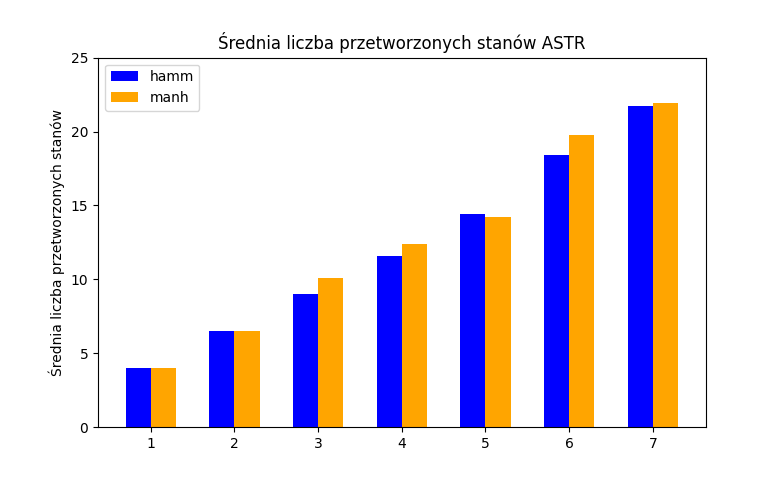
\includegraphics[width=\textwidth, height=55mm]{wykresy/astr3.png}
            \caption{Średnia liczba przetworzonych stanów}
        \end{figure}

        \begin{figure}[!htbp]
            \centering
            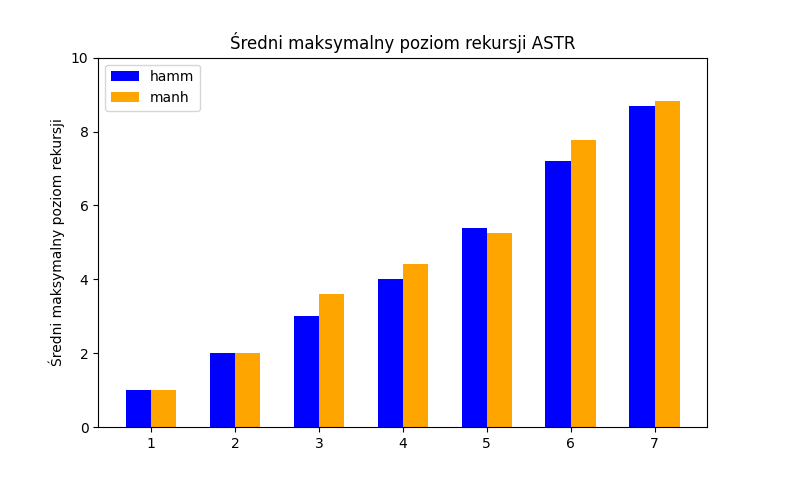
\includegraphics[width=\textwidth, height=55mm]{wykresy/astr4.png}
            \caption{Średni maksymalny poziom rekursji}
        \end{figure}

        \begin{figure}[!htbp]
            \centering
            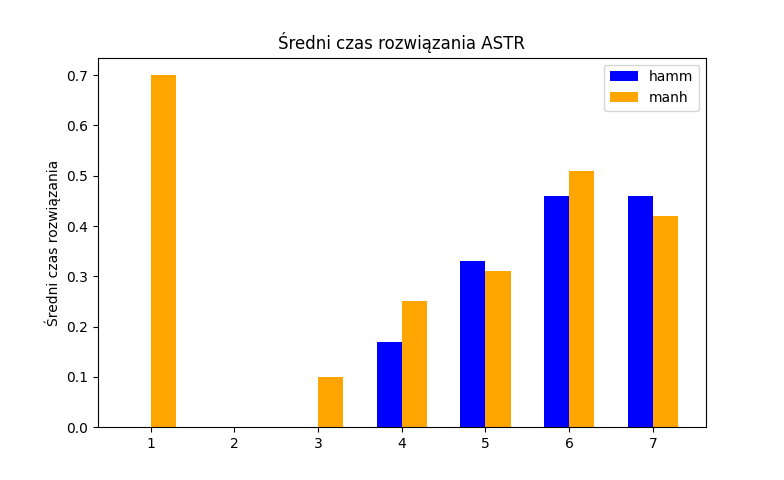
\includegraphics[width=\textwidth, height=55mm]{wykresy/astr5.png}
            \caption{Średni czas rozwiązania}
        \end{figure}
        \FloatBarrier
    }

    \section{Dyskusja} {
        \subsection{DFS}{
            Pod wszystkimi względami podany algorytm wypada najgorzej. Znalezienie rozwiązania zajmuje mu najdłużej.
        }
    
        \subsection{BFS}{
            Algorytm BFS posiada najkrótsze rozwiązania.
        }
    
        \subsection{ASTR}{
            W przypadku algorytmu ASTR najlepiej wypada liczba odwiedzonych i przetworzonych sygnałów. Trochę lepiej praktycznie pod każdym względem wypada parametr Hamminga. Nie w każdym przypadku udało się znaleźć rozwiązanie.
        }
    }

    \section{Wnioski} {
        \begin{itemize}
            \item Algorytm BFS znajduje najkrótsze rozwiązanie
            \item Metody heurystyczne nie zawsze potrafią znaleźć rozwiązanie
            \item Można stwierdzić, że trochę lepsza jest heurystyka Hamminga
            \item Najgorszym algorytmem jest DFS
            \item Metody heurystyczne nie zawsze potrafią znaleźć rozwiązanie
        \end{itemize}}
    
    \begin{thebibliography}{0}
        \bibitem{l2short} T. Oetiker, H. Partl, I. Hyna, E. Schlegl.
        \textsl{Nie za krótkie wprowadzenie do systemu \LaTeX2e}, 2007, dostępny
        online.
    \end{thebibliography}


\end{document}
